\begin{document}
\hypersetup{pageanchor=false}   % no PDF page anchors on the title/certificate pages (their numbers repeat later)
\begin{titlepage}
\doublespacing

\begin{center}
\par {\large \textbf{Mini Project-II Report}}\\
\end{center}

\begin{center}
	\par {\large \textbf{on}}
\end{center}

%\par~

\begin{center}
{\Large \textbf{Data Fusion and Ablation Study for Coffee Quality Assessment Using Electronic Nose Data}}
\end{center}

{\small
\begin{center}
\par \small {Submitted by}
\par \Large \textbf{Sai Aravind Chabala} \textbf{(23BDS075)}
\par \Large \textbf{Chevireddy Pothan Sai Reddy} \textbf{(23BDS017)}
\par \Large \textbf{Lingala Sahith Akash Manikanta} \textbf{(23BDS031)}
\par Under the guidance of
\par \large \textbf{Dr. Sunil C K}
\par \textbf{Assistant Professor}
\end{center}
}

\begin{figure}[h]
\begin{center}

\includegraphics[height=.80in]{iiIT-Dharwad-Logo-horizontal-500x154[1].png}
\end{center}
\end{figure}

\begin{center}
\par{\mbox {\small\textbf{DEPARTMENT OF DATA SCIENCE AND ARTIFICIAL INTELLIGENCE}}}
\noindent{\mbox{\small \textbf{ INDIAN INSTITUTE OF INFORMATION TECHNOLOGY
DHARWAD}}}\\
10/11/2026

\end{center}
\end{titlepage}


\newpage
\thispagestyle{empty}
%\mbox{}
\clearpage             %rest of the page is left blank in the title page
\thispagestyle{empty}  % to remove the page number from the empty page
\phantom{a}            %the particular page is left blank
%\vfill
\newpage
\thispagestyle{empty}

\begin{center}

	\emph{\huge{Certificate}}\\[2.5cm]
\end{center}
\normalsize This is to certify that the project, entitled \textbf{Data Fusion and Ablation Study for Coffee Quality Assessment Using Electronic Nose Data}, is a bonafide record of the Mini Project-II coursework presented by the students whose names are given below during the academic year 2026--2027 in partial fulfilment of the requirements of the degree of Bachelor of Technology in Data Science and Artificial Intelligence.\\[1.0cm]

\begin{table}[h]
	\centering
	\begin{tabular}{lr}
		Roll No & Names of Students \\ \\ \hline
		\\
		23BDS075 & Sai Aravind Chabala \\
		23BDS017 & Chevireddy Pothan Sai Reddy \\
		23BDS031 & Lingala Sahith Akash Manikanta \\
	\end{tabular}
\end{table}

\vfill


% Bottom of the page
\begin{flushright}
	Dr. Sunil C K\\
	(Project Supervisor )\\[1.5cm]
	%<Coordinator name here>\\
	%(Course Coordinator)\\
\end{flushright}

\newpage
\hypersetup{pageanchor=true}
\pagenumbering{roman}
\setcounter{page}{1}
\hypersetup{linkcolor=black}    % contents and lists stay black but are clickable
\tableofcontents
\newpage
\phantomsection
\listoffigures
\newpage
\phantomsection
\listoftables
\hypersetup{linkcolor=linkblue}



\newpage
\thispagestyle{empty}
%\mbox{}
\clearpage             %rest of the page is left blank in the title page
\thispagestyle{empty}  % to remove the page number from the empty page
\phantom{a}            %the particular page is left blank
%\vfill
\newpage

% Spacing for the main matter (set here so that the template preamble stays unchanged):
% tighter space around floats, lists and bibliography entries, and float placement that
% fills pages instead of leaving gaps. Section ends use \clearpage so floats stay in their section.
\setlength{\floatsep}{8pt plus 2pt minus 2pt}
\setlength{\textfloatsep}{10pt plus 2pt minus 4pt}
\setlength{\intextsep}{8pt plus 2pt minus 2pt}
\setlength{\abovecaptionskip}{4pt}
\setlength{\belowcaptionskip}{4pt}
\setlist{itemsep=1pt, parsep=0pt, topsep=3pt}
\setlength{\bibsep}{2pt plus 1pt}
\renewcommand{\topfraction}{0.9}
\renewcommand{\bottomfraction}{0.8}
\renewcommand{\textfraction}{0.07}
\renewcommand{\floatpagefraction}{0.75}
\setcounter{topnumber}{3}
\setcounter{bottomnumber}{2}
\setcounter{totalnumber}{5}

%%%***************************************************************************************
\section{Introduction}
\pagenumbering{arabic}

\subsection{Background and Motivation}

Coffee is graded for trade by trained tasters in \emph{cup tests}, which score aroma, flavour, acidity, body, balance and freedom from defects. Cup tests are partly subjective: Q-certified cuppers and a trained descriptive panel describing the same Colombian coffees agreed little \cite{didonfrancesco2014comparison}, and the total scores given by different cupping centres differ by about 3 points on the 100-point scale \cite{worku2016reproducibility}. Gas chromatography--mass spectrometry (GC-MS) identifies the volatile compounds behind coffee aroma precisely \cite{huang2007fingerprint} but is expensive and slow. Electronic noses (e-noses), arrays of broadly selective gas sensors followed by pattern recognition \cite{persaud1982analysis,gardner1999electronic}, are cheap and fast and respond to the whole volatile ``fingerprint'' of a sample \cite{wilson2009applications}.

Rodr\'{\i}guez et al.\ \cite{rodriguez2010electronic} classified Colombian coffee samples with an array of eight metal-oxide (MOX) gas sensors, using the variation between the maximum and minimum conductance of each sensor, principal component analysis (PCA) and a small neural network. The recordings were later released as a labelled data set of high-, average- and low-quality coffee \cite{rodriguezgamboa2020dataset}, which makes it possible to re-examine the method and to study how information from several sensors, or from several data sources, should be combined.

\subsection{Problem Statement, Objectives and Contributions}

Information from several sources can be fused at three levels \cite{hall1997introduction,borras2015data}: raw data can be combined before modelling (\emph{low level}), features extracted from each source can be concatenated (\emph{mid level}), or the decisions of separate models can be combined (\emph{high level}). This project determines which level works best for a small MOX sensor array and for related data sources, and how much of the accuracy reported on such small data sets survives a strict evaluation. Three public sources are used: \textbf{S1}, the coffee e-nose recordings \cite{rodriguezgamboa2020dataset}; \textbf{S2}, the SmellNet-Base gas-sensor data set with ingredient-level GC-MS vectors \cite{feng2026smellnet}; and \textbf{S3}, the Coffee Quality Institute (CQI) cupping database \cite{ledoux2018cqi}. The objectives are to:
\begin{enumerate}[label=O\arabic*.]
\item reproduce the reference pipeline \cite{rodriguez2010electronic} on S1 and compare the results with those reported;
\item compare low-, mid- and high-level fusion of the eight sensors of S1 (Experiment A);
\item test whether fusing S1 with S2 improves coffee quality classification (Experiment B);
\item compare the fusion levels on the attribute groups of S3 and use S3 to interpret the quality grades (Experiment C);
\item fuse gas-sensor data with ingredient-level GC-MS information in S2 without label leakage (Experiment D);
\item identify, through ablation studies, which components drive the results.
\end{enumerate}

The contributions are a reproduction of the reference method with repeated cross-validation alongside leave-one-out (LOO); a controlled comparison of the three fusion levels in which every fitted step is learned inside the training folds only; fifteen ablation studies, which show that a large part of the accuracy reachable on the public coffee data comes from the state of the sensors before the odour reaches them and that model selection by LOO is optimistic by about 4 points; and a demonstration that class-level chemical information cannot be fused at the input level without leaking the label. Section~\ref{sec:related} reviews related work, Section~\ref{sec:methods} describes the data and methods, Section~\ref{sec:results} presents and discusses the results, and Section~\ref{sec:conclusion} concludes the report.
\clearpage

%%%***************************************************************************************
\section{Related Work}
\label{sec:related}

\subsection{Electronic Noses for Coffee}

An e-nose combines partially selective chemical sensors with pattern recognition; Persaud and Dodd \cite{persaud1982analysis} showed that discrimination between many odours does not require highly specific receptors. The principles of e-nose design and data processing are covered in \cite{gardner1999electronic,marco2012signal}. The resistance of a MOX sensor falls in the presence of reducing gases, so the conductance $G = 1/R$ is the usual working quantity, and MOX sensors drift over time \cite{vergara2012chemical}. Coffee was one of the first e-nose applications \cite{gardner1992application}. Later work improved the classification of espresso brands through preprocessing \cite{pardo2000data}, classified coffees and predicted panel scores \cite{pardo2002coffee}, monitored ripening and roasting \cite{falasconi2005novel,romani2012evaluation}, detected adulteration \cite{brudzewski2012recognition} and estimated aroma intensity with a low-cost e-nose \cite{gonzalezviejo2021integrating}.

The reference work \cite{rodriguez2010electronic} used the A-NOSE (eight Figaro and FIS MOX sensors) on samples from the Almac\'{a}fe laboratory in C\'{u}cuta, Colombia. The variation between the maximum and minimum conductance of each sensor was mean-centred and used for PCA visualisation and for a feed-forward network with ten hidden neurons, trained by back-propagation with an adaptive learning rate and validated by LOO. The authors report 99.62\% of the variance in the first two principal components, 100\% accuracy for 16 measurements in four groups and 92.5\% for 35 measurements in nine categories.

\subsection{Machine Olfaction and Data Fusion}

SmellNet \cite{feng2026smellnet} records 50 substances on six days with six low-cost MOX channels and applies temporal differencing, sliding windows and standardisation before multilayer perceptron, convolutional, recurrent and Transformer models. It optionally aligns sensor embeddings with an ingredient-level GC-MS embedding during training through a symmetric contrastive loss, as in CLIP \cite{radford2021learning}, and reports that GC-MS supervision helps the weaker models most. Hall and Llinas \cite{hall1997introduction} describe data-, feature- and decision-level fusion, and Borr\`{a}s et al.\ \cite{borras2015data} review these levels for food quality assessment. Multi-level fusion of an e-nose and an e-tongue gave more accurate tea grading \cite{zhi2017framework}, and fused e-nose and e-tongue data were best for robusta coffee \cite{dong2017differentiation}; the benefit of high-level fusion depends, however, on the correlation structure of the combined models \cite{doeswijk2011increase}. Stacked generalisation \cite{wolpert1992stacked} learns how to combine models from their out-of-sample predictions.

\subsection{Cupping Scores and Validation Practice}

The specialty-coffee cupping methodology combines a set of sensory attribute scores into a numeric quality score \cite{revi2019coffee}; cupping and descriptive analysis provide different information \cite{didonfrancesco2014comparison}, and scores differ between cupping centres \cite{worku2016reproducibility}. When classifier parameters are tuned by the same cross-validation that estimates their error, the estimate is optimistically biased, which nested cross-validation avoids \cite{varma2006bias,cawley2010overfitting}, and leakage of target information is a common source of inflated results \cite{kaufman2012leakage}. McNemar's test \cite{dietterich1998approximate} and the Wilcoxon signed-rank test \cite{demsar2006statistical} are recommended for comparing classifiers.

Table~\ref{tab:related} summarises the most relevant studies. Coffee e-nose studies use small sample sets, rarely report validation that is independent of the measurement session, and do not compare the fusion levels on the same data under one protocol; this project addresses that gap.

\begin{table}[!htbp]
\centering
\caption[Summary of the most relevant related work]{Summary of the most relevant related work (results as reported by the authors).}
\label{tab:related}
\footnotesize
\begin{tabularx}{\textwidth}{>{\raggedright\arraybackslash}p{2.9cm}>{\raggedright\arraybackslash}X>{\raggedright\arraybackslash}X>{\raggedright\arraybackslash}p{3.4cm}}
\toprule
\textbf{Work} & \textbf{Data} & \textbf{Method} & \textbf{Reported result} \\
\midrule
Rodr\'{\i}guez et al.\ \cite{rodriguez2010electronic} & Colombian coffee; 16 and 35 measurements & 8 MOX sensors; conductance variation, PCA, MLP (10 hidden); LOO & 100\% (4 groups), 92.5\% (9 categories) \\
Pardo and Sberveglieri \cite{pardo2002coffee} & 2 groups of 7 coffees & Thin-film sensors; PCA, MLP; regression of panel scores & Above 90\% classification \\
Gonzalez Viejo et al.\ \cite{gonzalezviejo2021integrating} & 9 commercial coffees in triplicate & Low-cost e-nose; neural networks & 98\% (intensity class) \\
Zhi et al.\ \cite{zhi2017framework} & Tea, 4 grades & E-nose + e-tongue; feature- and decision-level fusion & More accurate grading with multi-level fusion \\
Feng et al.\ \cite{feng2026smellnet} & 50 substances, 6 days & Windows; MLP, CNN, LSTM, Transformer; contrastive GC-MS & 56.1\% $\rightarrow$ 63.3\% (Transformer) \\
Varma and Simon \cite{varma2006bias} & Simulated data & Cross-validation for model selection & Non-nested CV is optimistic \\
\bottomrule
\end{tabularx}
\end{table}
\clearpage

%%%***************************************************************************************
\section{Data and Methods}
\label{sec:methods}

\subsection{Data Sets}

\textbf{S1: coffee e-nose data.} S1 \cite{rodriguezgamboa2020dataset} contains 58 recordings of roasted, ground Colombian coffee labelled high (HQ, $n = 20$), average (AQ, $n = 10$) and low quality (LQ, $n = 28$). Each recording holds the resistance (k$\Omega$) of the eight A-NOSE sensors (Table~\ref{tab:sensors}) sampled at 1~Hz for 300~s, and all files are complete. Predicting the majority class gives 48.3\% accuracy, and the public labels do not map onto the four groups and nine categories of \cite{rodriguez2010electronic}.

\textbf{S2: SmellNet-Base.} S2 \cite{feng2026smellnet} contains 50 substances, each recorded on six days at 1~Hz (300 sessions; median length 600~s, range 517--867~s), with six uncalibrated channels: NO$_2$, C$_2$H$_5$OH, VOC and CO (Grove Multichannel Gas Sensor V2), alcohol (MQ-3) and LPG (MQ-5). Each substance has one GC-MS vector derived from the FooDB database in two encodings: binned mass spectra (460 dimensions) and elemental composition (17 dimensions). These vectors describe ingredients, not sessions, and are therefore class-level information. Days 1--5 form the official training set and day 6 the test set.

\textbf{S3: CQI database.} After the removal of one empty review, S3 \cite{ledoux2018cqi} contains 1,338 reviews (1,310 arabica and 28 robusta; 183 from Colombia) with ten sensory scores (group G1), physical and bean data (G2: moisture, category-one and category-two defects, quakers, colour, processing method, species) and origin data (G3: country, region, altitude). The robusta columns were renamed to their arabica equivalents and altitudes above 5,000~m were treated as missing. The total cup score equals the sum of the ten G1 scores for 95.1\% of the reviews (maximum difference 0.5 points). S3 shares no samples with S1 or S2, and no samples were paired across data sets. Table~\ref{tab:datasets} summarises the three sources.

\begin{table}[!htbp]
\centering
\caption[Sensors of the A-NOSE]{Sensors of the A-NOSE \cite{rodriguez2010electronic}.}
\label{tab:sensors}
\small
\begin{tabular}{llll}
\toprule
\textbf{Sensor} & \textbf{Stated application} & \textbf{Sensor} & \textbf{Stated application} \\
\midrule
SP-12A & Flammable gases & SP-AQ3 & Air quality control \\
SP-31 & Organic solvents & TGS-823 & Combustible gases \\
TGS-813 & Combustible gas & ST-31 & Organic solvents \\
TGS-842 & Methane, natural gas & TGS-800 & Air quality, smoke, benzene \\
\bottomrule
\end{tabular}
\end{table}

\begin{table}[!htbp]
\centering
\caption[Summary of the three data sources]{Summary of the three data sources.}
\label{tab:datasets}
\footnotesize
\begin{tabularx}{\textwidth}{>{\raggedright\arraybackslash}p{2.4cm}>{\raggedright\arraybackslash}X>{\raggedright\arraybackslash}X>{\raggedright\arraybackslash}X}
\toprule
 & \textbf{S1: coffee e-nose} & \textbf{S2: SmellNet-Base} & \textbf{S3: CQI database} \\
\midrule
Type & MOX sensor time series & MOX sensor time series + GC-MS vectors & Tabular cupping scores and metadata \\
Size & 58 recordings & 300 sessions (50 substances $\times$ 6 days) & 1,338 reviews \\
Channels or attributes & 8 sensors, 300~s at 1~Hz (k$\Omega$) & 6 channels, 517--867~s at 1~Hz; GC-MS 460 or 17 dimensions & 10 sensory, 7 physical, 3 origin attributes \\
Labels & HQ 20, AQ 10, LQ 28 & 50 substances & Total-score tertiles: HQ 481, AQ 425, LQ 432 \\
Role & Reproduction, Experiment A & Experiments B and D & Experiment C \\
\bottomrule
\end{tabularx}
\end{table}

\subsection{Signal Representation and Features}

The resistance $R_s(t)$ of sensor $s$ is converted to the conductance $G_s(t) = 1/R_s(t)$, $t = 1, \dots, 300$. Since the reference work does not give the formula of its static parameter, the absolute and the relative variation were implemented:
\begin{equation}
\Delta G_s = \max_t G_s(t) - \min_t G_s(t), \qquad \Delta G_s^{\mathrm{rel}} = \Delta G_s / \min_t G_s(t).
\end{equation}
For the fusion experiments, 15 features were computed per sensor (Table~\ref{tab:features}), where $b_s$ is the baseline (the mean of the first 20~s, before the odour arrives) and $t^{*}_s = \arg\max_t |G_s(t) - b_s|$. The features depend on a single recording only and therefore carry no information across folds.

\begin{table}[!htbp]
\centering
\caption[Features computed for each sensor]{The 15 features computed for each sensor.}
\label{tab:features}
\footnotesize
\begin{tabular}{lll}
\toprule
\textbf{No.} & \textbf{Feature} & \textbf{Definition} \\
\midrule
1 & Baseline & $b_s = \frac{1}{20}\sum_{t=1}^{20} G_s(t)$ \\
2--4 & Maximum, minimum, range & $\max_t G_s(t)$, $\min_t G_s(t)$, $\Delta G_s$ \\
5 & Relative peak change & $(G_s(t^{*}_s) - b_s)/|b_s|$ \\
6--7 & Mean, standard deviation & over $t = 1, \dots, 300$ \\
8 & Area & $\sum_t (G_s(t) - b_s)$ (trapezoidal rule) \\
9--10 & Maximum and minimum slope & $\max_t$ and $\min_t$ of $G_s(t+1) - G_s(t)$ \\
11 & Time of peak & $t^{*}_s$ \\
12 & Final value & mean of the last 10~s \\
13--15 & Spectral magnitudes & $|\mathcal{F}_k|/T$ of $G_s - b_s$ for $k = 1, 2, 3$ \\
\bottomrule
\end{tabular}
\end{table}

\subsection{Fusion Schemes}

Let $\mathbf{G} = [G_1, \dots, G_8]$ be the curves of a recording, $\phi(G_s) \in \mathbb{R}^{15}$ the features of sensor $s$ and $K$ the number of classes. The three fusion levels (Figure~\ref{fig:levels}) are:
\begin{itemize}
\item \textbf{Low level:} $\mathbf{x}^{\mathrm{low}} = \mathrm{vec}(\mathbf{G}) \in \mathbb{R}^{2400}$ is standardised, projected onto 10 principal components and classified. A second low-level model is a one-dimensional CNN with the eight sensors as input channels (16 and 32 filters of width 7 and 5 with batch normalisation, max pooling, global average pooling and dropout 0.3), optionally trained on sliding 250-s windows (stride 10~s) with test-time averaging over the windows of a recording.
\item \textbf{Mid level:} $\mathbf{x}^{\mathrm{mid}} = [\phi(G_1); \dots; \phi(G_8)] \in \mathbb{R}^{120}$ is standardised and classified.
\item \textbf{High level:} one classifier $f_s$ per sensor gives class probabilities $\mathbf{p}_s$, which are combined by majority vote (ties broken by the mean probability), by the mean $\bar{\mathbf{p}} = \frac{1}{S}\sum_s \mathbf{p}_s$, by a weighted mean or by stacking:
\begin{equation}
\mathbf{p}^{w} = \sum_{s=1}^{S} w_s \mathbf{p}_s, \quad w_s \propto \max(a_s - 1/K, \epsilon), \qquad \mathbf{p}^{\mathrm{stack}} = g\left([\log \mathbf{p}_1; \dots; \log \mathbf{p}_S]\right),
\end{equation}
where $a_s$ is the inner-CV accuracy of $f_s$ and $g$ is a multinomial logistic regression trained on the inner out-of-fold probabilities \cite{wolpert1992stacked}.
\end{itemize}

\begin{figure}[!htbp]
\centering
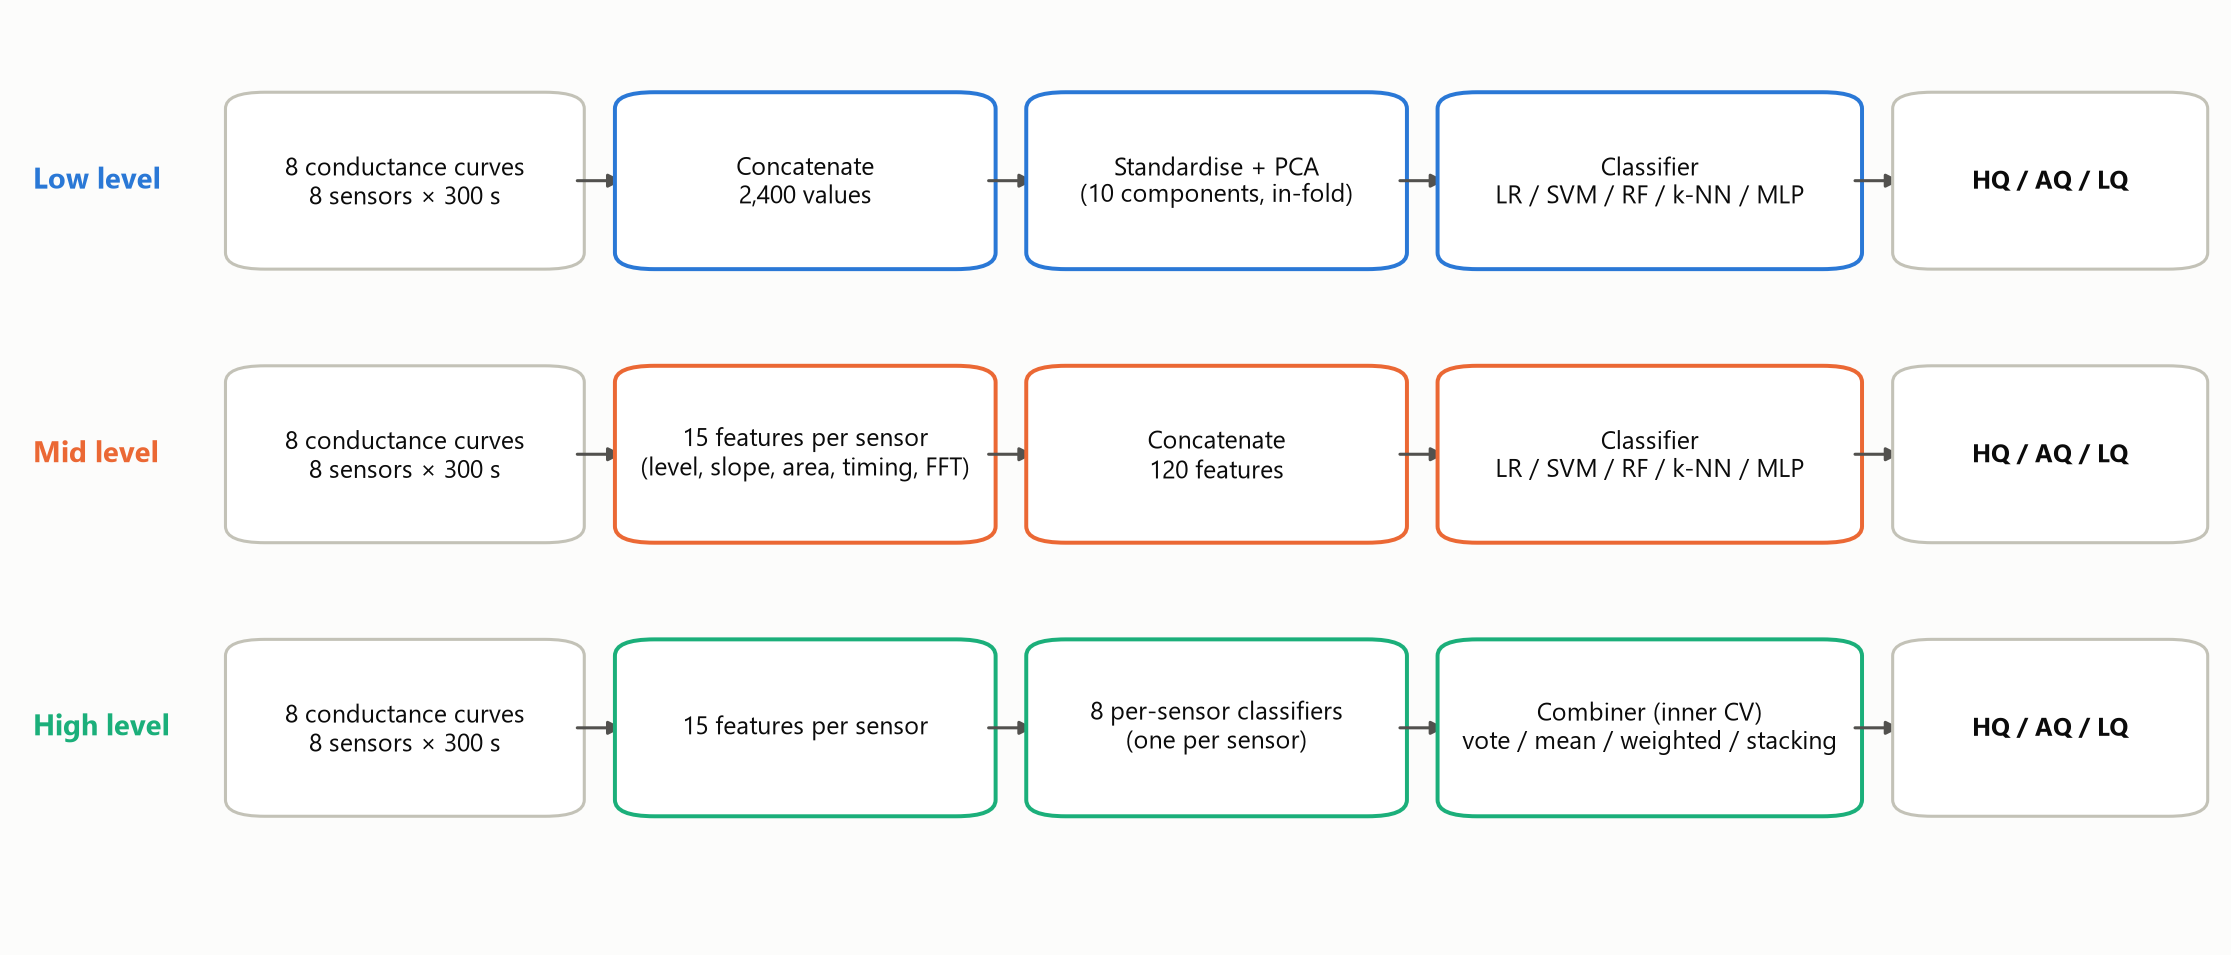
\includegraphics[width=0.9\textwidth]{figures/fig_fusion_levels.png}
\caption[The three fusion levels compared in Experiment A]{The three fusion levels compared in Experiment A.}
\label{fig:levels}
\end{figure}

\textbf{Experiment A} treats each sensor of S1 as a source and compares the three fusion levels with five classifier families on the conductance curves.

\textbf{Experiment B} fuses S1 with S2. The sources were harmonised by (i) converting S1 to conductance so that both signals rise with gas, (ii) cutting both to the first 300~s and (iii) z-scoring every channel of every recording. Because S1 has eight channels and S2 six, channel-agnostic models were used. B1 (low level) applies a shared univariate CNN encoder to every channel and pools the channel embeddings by their mean and maximum. B2 (mid level) aggregates the per-channel features across channels, $\psi(\mathbf{x}) = [\mathrm{mean}_c\,\phi(x_c); \mathrm{std}_c\,\phi(x_c); \max_c \phi(x_c); \min_c \phi(x_c)] \in \mathbb{R}^{60}$. B3 (high level) combines a model trained on S1 alone with a model trained on S1 + S2. B1 and B2 are trained on the 3 coffee classes plus the 50 SmellNet substances and evaluated only on held-out S1 recordings, predicting $\hat{y} = \arg\max_{k \in \{\mathrm{HQ}, \mathrm{AQ}, \mathrm{LQ}\}} p_k(\mathbf{x})$; S2 enters only the training side.

\textbf{Experiment C} predicts the tertile of the CQI total score (LQ below 81.67, AQ 81.67--83.17 and HQ above 83.17 points). Because the total is the sum of G1, G1 is reported only as an upper bound and the fusion study uses G2 and G3: C1 concatenates their encoded columns, C2 concatenates per-group PCA embeddings (5 components for G2 and 10 for G3) and C3 combines one model per group. Imputation, one-hot encoding (categories with at least 10 reviews) and PCA are fitted inside each training fold.

\textbf{Experiment D} uses the multilayer-perceptron backbone of SmellNet (two hidden layers of 256 units on time-pooled windows), the setting in which \cite{feng2026smellnet} reports the clearest benefit from GC-MS supervision. Following \cite{feng2026smellnet}, each session is offset by its first sample, optionally differenced, $\Delta x_t = x_t - x_{t-p}$ with $p \in \{0, 25\}$, cut after splitting into windows of $w \in \{50, 100\}$ samples (stride $w/2$) and standardised with training statistics. Four systems were compared, all of which receive sensor data only at test time. D0 is trained with the cross-entropy loss $\mathcal{L}_{\mathrm{CE}}$. D1 aligns a sensor encoder $h$ with a GC-MS encoder $g$ through the symmetric contrastive loss
\begin{equation}
\mathcal{L}_{\mathrm{con}} = -\frac{1}{2B} \sum_{i=1}^{B} \left[ \log \frac{e^{s_{ii}/\tau}}{\sum_{j} e^{s_{ij}/\tau}} + \log \frac{e^{s_{ii}/\tau}}{\sum_{j} e^{s_{ji}/\tau}} \right], \qquad s_{ij} = \cos\left(h(\mathbf{x}_i), g(\mathbf{c}_{y_j})\right),
\end{equation}
with $\tau = 0.07$ and batches of distinct ingredients, and classifies a window as the most similar of all 50 ingredient embeddings. D2 minimises $\mathcal{L}_{\mathrm{CE}} + \lambda \mathcal{L}_{\mathrm{con}}$ with $\lambda \in \{0.1, 0.5, 1\}$. D3 combines D0 and D1 as $\mathbf{p} = \alpha\,\mathrm{softmax}(f(\mathbf{x})) + (1-\alpha)\,\mathrm{softmax}(\mathbf{s}(\mathbf{x})/\tau)$ with $\alpha \in \{0, 0.25, 0.5, 0.75, 1\}$. Low-level fusion is not valid here: the GC-MS vector of a sample is a function of its label, so concatenating it at test time would require knowing the answer (Section~\ref{sec:expD}).

\subsection{Classifiers, Training and Evaluation}

The classifiers were logistic regression ($C = 1$), an RBF support vector machine whose $C \in \{1, 10, 100\}$ was chosen by a three-fold grid search inside each training fold (nested cross-validation), a random forest (300 trees), $k$-nearest neighbours ($k = 5$) and an MLP with one hidden layer of 10 units, the size used in \cite{rodriguez2010electronic}. Class weights were balanced where supported; gradient boosting was added for S3 and an MLP with 64 hidden units for Experiment B. The CNNs were trained with AdamW (learning rate $3 \times 10^{-3}$, weight decay $10^{-3}$, batch size 16) for 150 epochs, or 60 epochs for the windowed variant. In Experiment D, Adam (batch size 32) was used for at most 90 epochs with early stopping after 25 epochs without improvement on the validation day, on which the learning rate ($3 \times 10^{-4}$, $10^{-3}$ or $3 \times 10^{-3}$), $\lambda$ and $\alpha$ were also selected. For the reproduction, the reference network (ten hidden neurons, back-propagation with an adaptive learning rate) was implemented with stochastic gradient descent (adaptive rate starting at 0.05, momentum 0.9) and with Adam, under three input scalings (none, mean-centring as in the reference work, autoscaling) and with a three-unit softmax output.

On S1, leave-one-out (for comparability with \cite{rodriguez2010electronic}) and stratified five-fold cross-validation repeated ten times (five times for the ablations) were used; on S3, stratified five-fold cross-validation repeated five times; on S2, days 1--4 for training, day 5 for selecting the hyper-parameters and the training epoch, and the official test day 6 for evaluation, with the seeds 42, 7 and 123. Splits are made at the level of whole recordings, and everything fitted to data is fitted on the training part of each fold only (Algorithm~\ref{alg:cv}). Accuracy, balanced accuracy and macro-F1 are reported as the mean $\pm$ standard deviation over repeats or seeds:
\begin{equation}
\mathrm{Acc} = \frac{1}{N}\sum_{i=1}^{N} \mathbf{1}[\hat{y}_i = y_i], \qquad \mathrm{BAcc} = \frac{1}{K}\sum_{k=1}^{K} \mathrm{Rec}_k, \qquad \mathrm{F1}_{\mathrm{macro}} = \frac{1}{K}\sum_{k=1}^{K} F_{1,k}.
\end{equation}
Paired comparisons use the Wilcoxon signed-rank test over the repeats \cite{demsar2006statistical} and McNemar's exact test on the 58 LOO predictions \cite{dietterich1998approximate}, $p = \min\{1, 2\Pr[X \leq \min(n_{01}, n_{10})]\}$ with $X \sim \mathrm{Binomial}(n_{01} + n_{10}, 0.5)$, where $n_{01}$ and $n_{10}$ count the recordings classified correctly by only one of the two models.

\begin{algorithm}[!htbp]
\caption[Leakage-free repeated cross-validation with high-level fusion]{Leakage-free repeated cross-validation with high-level fusion}
\label{alg:cv}
\begin{algorithmic}[1]
\REQUIRE recordings $\{(\mathbf{G}_i, y_i)\}_{i=1}^{N}$, sources $s = 1, \dots, S$, repeats $R$
\FOR{$r = 1$ \TO $R$}
\STATE split the recordings into 5 stratified folds with seed $r$
\FOR{each fold $k$}
\STATE compute the per-recording features $\phi(G_{i,s})$ (no fitted parameters)
\STATE run a 5-fold inner cross-validation on the training part: fit the per-source scaler and classifier $f_s$ (SVM $C$ chosen by an inner grid search) and collect out-of-fold probabilities
\STATE derive the combiner weights $w_s$ and fit the stacking meta-learner $g$ on the out-of-fold probabilities
\STATE refit every $f_s$ on the whole training part, predict the test fold and combine the predictions
\ENDFOR
\STATE compute accuracy, balanced accuracy and macro-F1 of repeat $r$
\ENDFOR
\RETURN mean and standard deviation over the $R$ repeats
\end{algorithmic}
\end{algorithm}

\subsection{Ablation Design and Implementation}

Each ablation changes one factor and keeps everything else fixed; for S1, one reference model per level is used (low: curves with PCA and logistic regression; mid: features with SVM; high: per-sensor logistic regression with stacking). AB1 removes each sensor and uses each sensor alone; AB2 varies the signal duration (30--300~s); AB3 varies the representation ($R$, $G$, $R/R_0$, $G/G_0$, a per-recording z-score, differencing); AB4 removes each feature type; AB5 and AB6 compare combiners and classifier families; AB7 compares LOO with repeated cross-validation; AB8 varies the amount of S2 data (10--100\% of the sessions) and each harmonisation step; AB9 removes each CQI group; AB10 tests window augmentation; and AB11--AB15 cover Experiment D (with versus without GC-MS, the GC-MS encoding, window size and differencing, masking of each channel at test time, and $\lambda$ and $\alpha$). All code was written in Python 3.12 (NumPy 2.5.4, pandas 3.1.1, scikit-learn 1.9.1, SciPy 1.18.1, PyTorch 2.15.0) and run on a laptop with an Intel Core i7-1180G7 processor and 16~GB of memory. Random seeds were fixed, and every fold was stored with its configuration and per-sample predictions, from which all tables and figures are regenerated.
\clearpage

%%%***************************************************************************************
\section{Results and Discussions}
\label{sec:results}

\subsection{Exploratory Analysis and Reproduction of the Reference Method}

Figure~\ref{fig:curves} shows the class-mean responses: a flat baseline, a sharp drop in resistance when the coffee headspace reaches the sensors, and a slow recovery. HQ is clearly separated, while AQ and LQ nearly overlap on seven of the eight sensors. The baseline, which is measured before the coffee arrives, already differs between the classes (SP-12A, first 20~s: 46.4, 33.9 and 38.7~k$\Omega$ for HQ, AQ and LQ). Table~\ref{tab:onset} gives the first second at which each sensor falls 5\% below its baseline: the six fast sensors respond between 32 and 34~s in every recording and none before 30~s, while SP-12A never falls 5\% below its starting level in 32 of the 58 recordings.

\begin{figure}[!htbp]
\centering
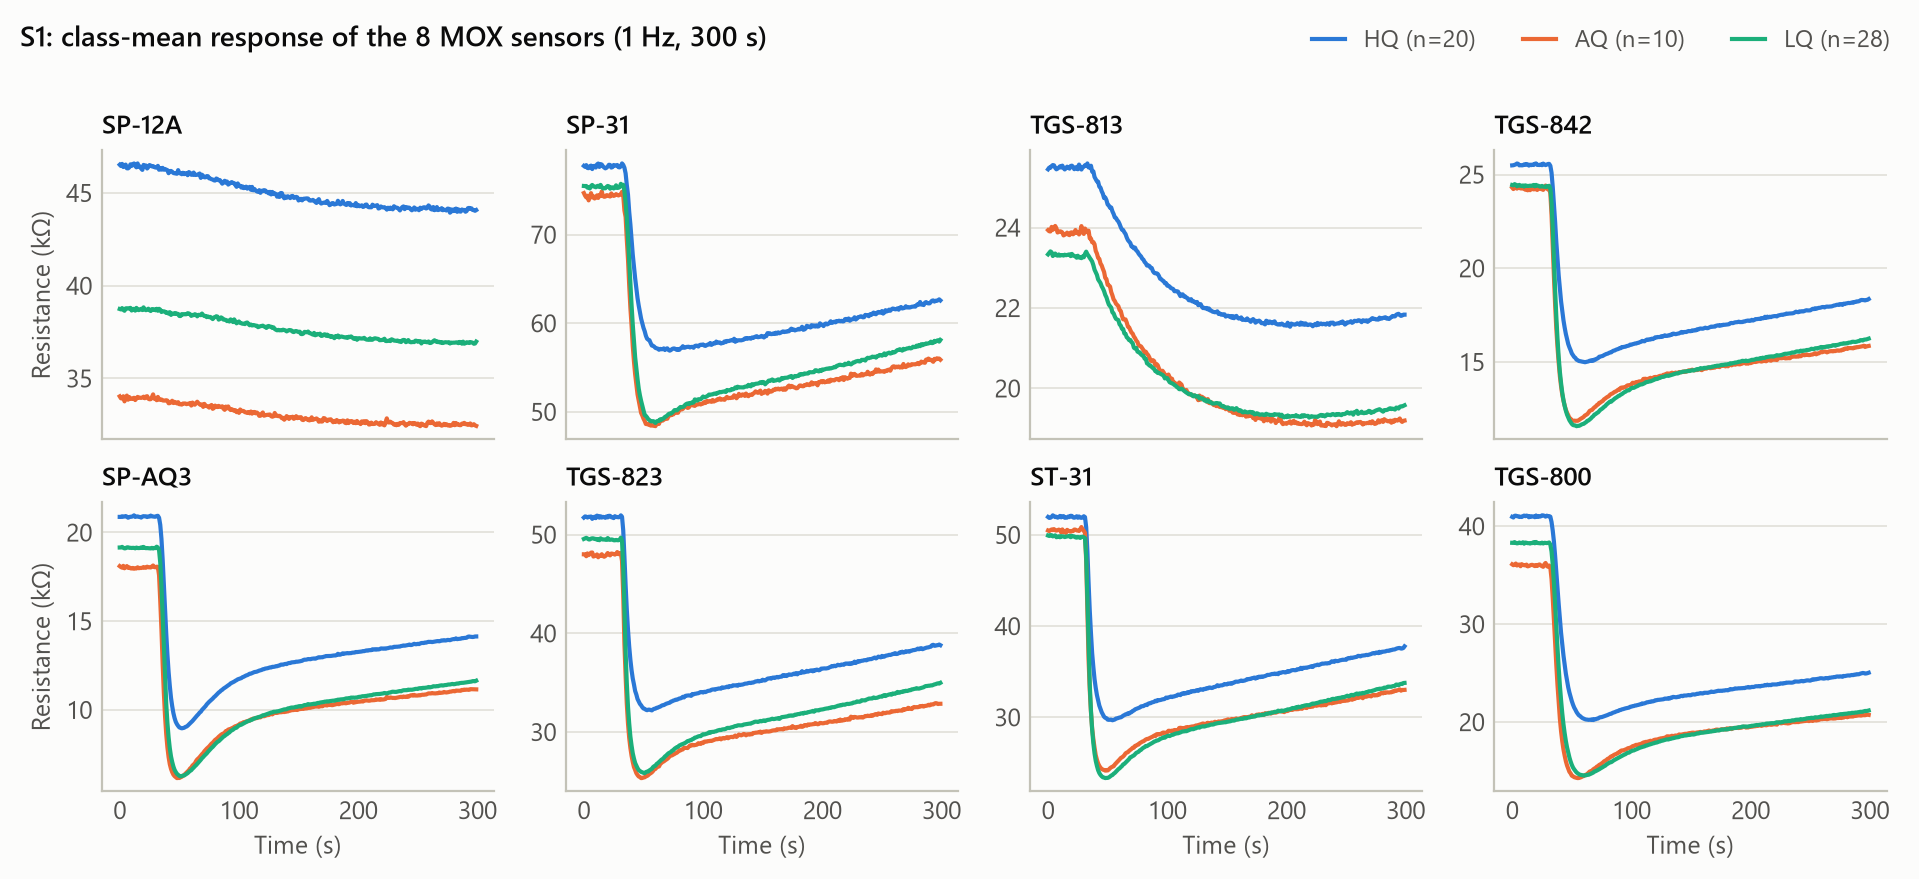
\includegraphics[width=\textwidth]{figures/fig1_s1_sensor_curves.png}
\caption[Class-mean resistance of the eight sensors of S1]{Class-mean resistance of the eight sensors of S1 (1~Hz, 300~s).}
\label{fig:curves}
\end{figure}

\begin{table}[!htbp]
\centering
\caption[Onset of the odour response in S1]{Onset of the odour response in S1: first second at which the resistance falls more than 5\% below the mean of the first 20~s.}
\label{tab:onset}
\footnotesize
\begin{tabular}{lcccc}
\toprule
\textbf{Sensor} & \textbf{Median onset (s)} & \textbf{Min (s)} & \textbf{Max (s)} & \textbf{Recordings without a 5\% drop} \\
\midrule
SP-12A & 300 & 78 & 300 & 32 \\
SP-31 & 37 & 35 & 41 & 0 \\
TGS-813 & 53 & 42 & 62 & 0 \\
TGS-842 & 34 & 33 & 37 & 0 \\
SP-AQ3 & 35 & 33 & 40 & 0 \\
TGS-823 & 34 & 33 & 35 & 0 \\
ST-31 & 33 & 32 & 34 & 0 \\
TGS-800 & 35 & 33 & 42 & 0 \\
\bottomrule
\end{tabular}

\end{table}

As in \cite{rodriguez2010electronic}, the PCA of the static parameter separates HQ while AQ and LQ overlap (Figure~\ref{fig:pca}). With mean-centring, the first two components explain 99.55\% of the variance, close to the reported 99.62\%; this mainly reflects scale, since SP-AQ3 alone has a loading of 0.85 on PC1 and after autoscaling the share falls to 93.58\%. Table~\ref{tab:baseline} reports the ten-hidden-unit network. Implemented literally (absolute $\Delta G$, mean-centring, gradient descent with an adaptive learning rate), it barely leaves the majority class (51.7\% LOO against 48.3\%), because the absolute conductance variations are tiny (about 0.001--0.2~mS). The scale-free relative parameter reaches 83.3\% LOO and 79.1\% in repeated cross-validation, against the 100\% and 92.5\% reported on 16 and 35 measurements with four and nine classes.

\begin{figure}[!htbp]
\centering
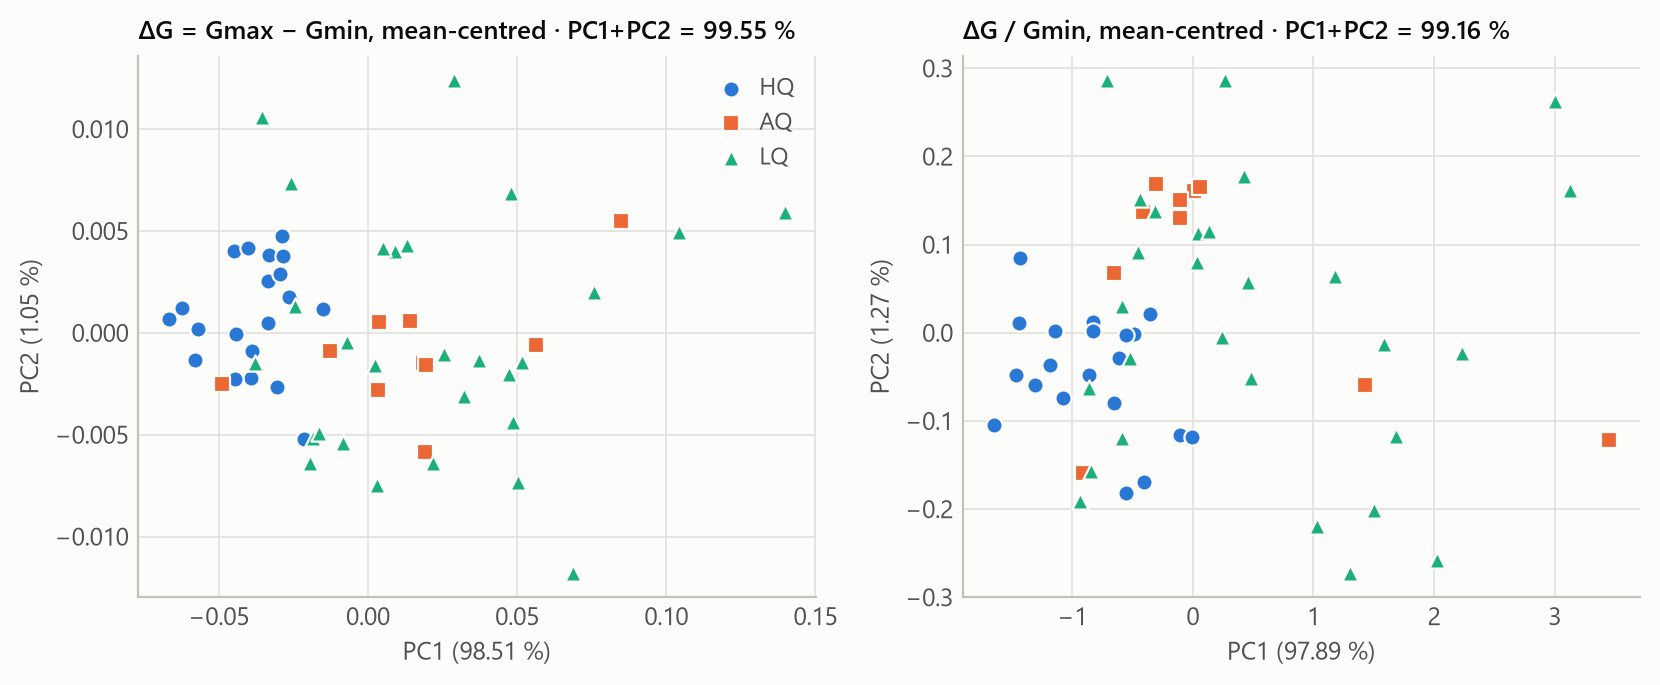
\includegraphics[width=0.9\textwidth]{figures/fig2_pca_static_parameter.png}
\caption[PCA of the mean-centred static parameter of S1]{PCA of the mean-centred static parameter of S1. Left: absolute variation $\Delta G$; right: relative variation $\Delta G/G_{\min}$.}
\label{fig:pca}
\end{figure}

\begin{table}[!htbp]
\centering
\caption[Reproduction of the reference pipeline on S1]{Reproduction of the reference pipeline on S1 (MLP with 10 hidden units; mean $\pm$ standard deviation over three initialisations for LOO and over ten repeats for five-fold cross-validation).}
\label{tab:baseline}
\footnotesize
\begin{tabular}{lllccc}
\toprule
\textbf{Static parameter} & \textbf{Input scaling} & \textbf{Solver} & \textbf{LOO acc. (\%)} & \textbf{10$\times$5-fold acc. (\%)} & \textbf{Macro-F1} \\
\midrule
$\Delta$G = Gmax $-$ Gmin & none & SGD & 51.1 $\pm$ 6.5 & 55.5 $\pm$ 5.8 & 0.347 \\
$\Delta$G = Gmax $-$ Gmin & none & Adam & 69.0 $\pm$ 1.7 & 69.8 $\pm$ 4.7 & 0.534 \\
$\Delta$G = Gmax $-$ Gmin & mean-centring & SGD & 51.7 $\pm$ 7.5 & 54.7 $\pm$ 5.7 & 0.334 \\
$\Delta$G = Gmax $-$ Gmin & mean-centring & Adam & 71.8 $\pm$ 3.6 & 70.7 $\pm$ 3.9 & 0.556 \\
$\Delta$G = Gmax $-$ Gmin & autoscaling & SGD & 70.7 $\pm$ 3.4 & 73.4 $\pm$ 3.9 & 0.684 \\
$\Delta$G = Gmax $-$ Gmin & autoscaling & Adam & 75.3 $\pm$ 2.0 & 74.0 $\pm$ 4.2 & 0.687 \\
$\Delta$G / Gmin & none & SGD & 72.4 $\pm$ 3.0 & 73.3 $\pm$ 2.7 & 0.622 \\
$\Delta$G / Gmin & none & Adam & 71.8 $\pm$ 5.5 & 73.8 $\pm$ 4.7 & 0.699 \\
$\Delta$G / Gmin & mean-centring & SGD & 83.3 $\pm$ 1.0 & 79.1 $\pm$ 3.1 & 0.734 \\
$\Delta$G / Gmin & mean-centring & Adam & 79.3 $\pm$ 1.7 & 78.3 $\pm$ 2.8 & 0.721 \\
$\Delta$G / Gmin & autoscaling & SGD & 81.0 $\pm$ 1.7 & 80.0 $\pm$ 4.2 & 0.764 \\
$\Delta$G / Gmin & autoscaling & Adam & 78.7 $\pm$ 2.6 & 79.7 $\pm$ 4.4 & 0.754 \\
\bottomrule
\end{tabular}

\end{table}

\subsection{Experiment A: Fusion of the Eight Sensors}

With conductance signals, low-level fusion is the most accurate (Figure~\ref{fig:summary}, Table~\ref{tab:expA}): the curves with PCA and logistic regression reach 91.7 $\pm$ 2.1\% (LOO 93.1\%) and the CNN 88.8\% (89.1\% with windows), against 86.7 $\pm$ 2.2\% for mid-level fusion (SVM) and 84.3 $\pm$ 2.9\% for high-level fusion (SVM with stacking). Over the ten repeats the low level beats the mid and high levels (Wilcoxon $p = 0.002$ in both cases), while mid and high do not differ ($p = 0.25$); on the 58 LOO predictions McNemar's test finds no significant difference (all $p > 0.2$), which shows how little a single LOO pass can resolve. Stacking is the best combiner for both per-sensor model families (Table~\ref{tab:expAhigh}), whereas voting and averaging over eight individually weak sensors lose information \cite{doeswijk2011increase}. HQ is almost never missed (recall 0.94--1.00), whereas the smallest class, AQ, causes most errors: 51--75\% of all errors are AQ/LQ confusions, and most of the advantage of low-level fusion comes from AQ (recall 0.80 against 0.57 at the mid and 0.54 at the high level).

\begin{figure}[!htbp]
\centering
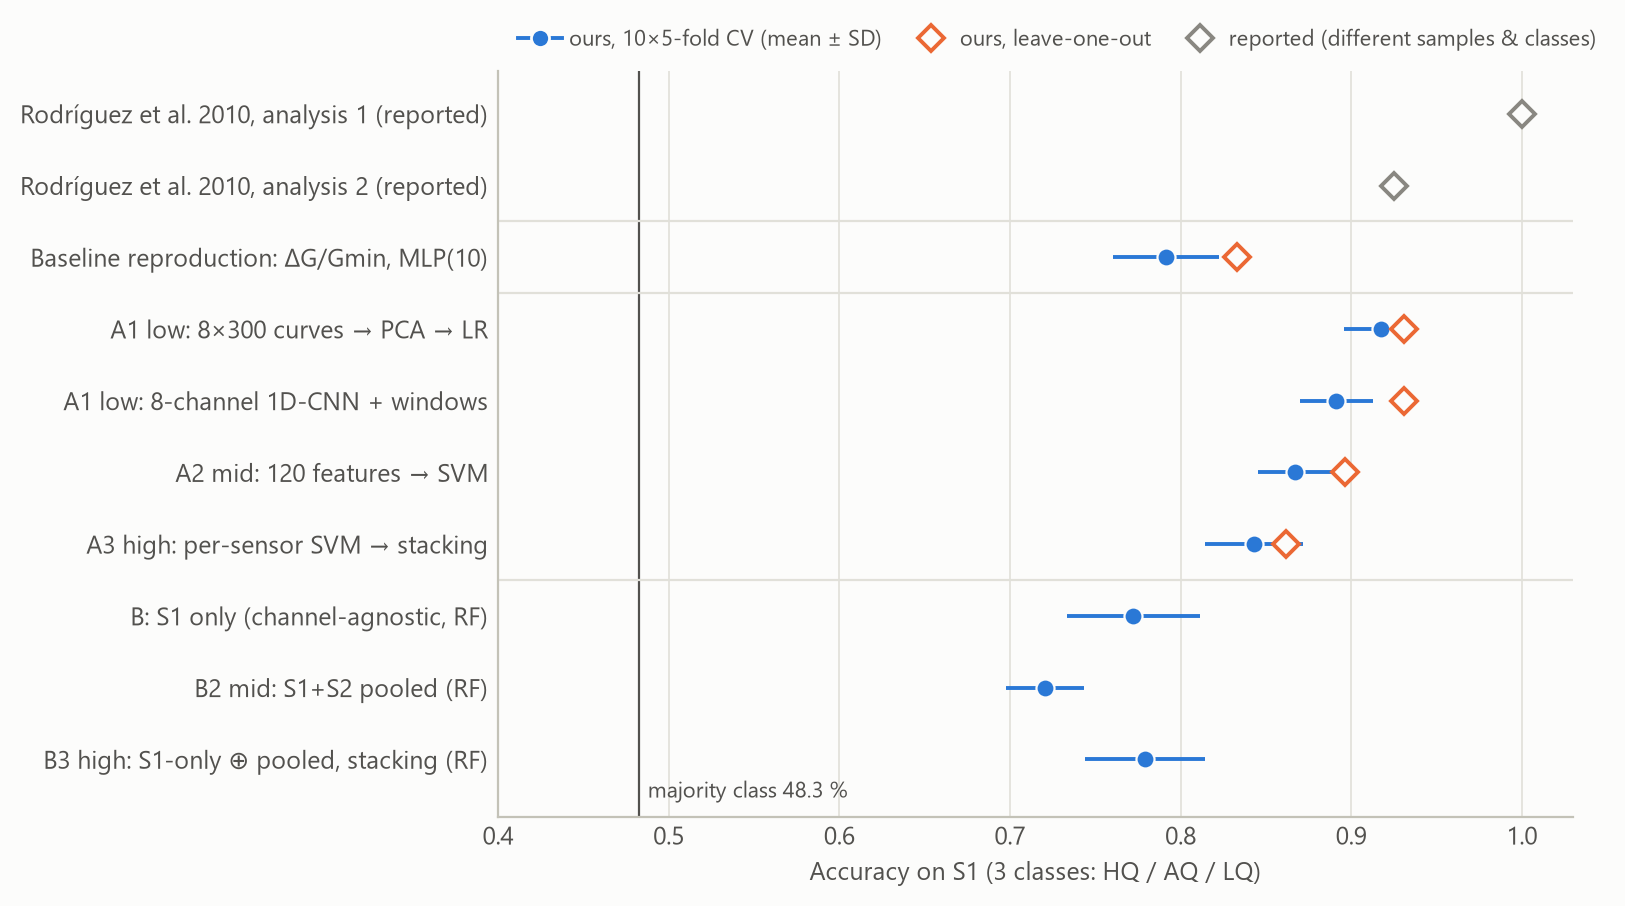
\includegraphics[width=0.8\textwidth]{figures/fig3_fusion_summary.png}
\caption[Accuracy on S1 of the baseline and the fusion schemes]{Accuracy on S1 of the reproduced baseline, the three fusion levels and the fusion with S2. Dots with bars: repeated five-fold cross-validation (mean $\pm$ standard deviation); hollow diamonds: LOO; grey diamonds: values reported in \cite{rodriguez2010electronic} for different samples and classes.}
\label{fig:summary}
\end{figure}

\begin{table}[!htbp]
\centering
\caption[Experiment A: accuracy by classifier and fusion level]{Experiment A: accuracy (\%) by classifier and fusion level (ten repeats of five-fold cross-validation, mean $\pm$ standard deviation, and LOO).}
\label{tab:expA}
\footnotesize
\begin{tabular}{lcccc}
\toprule
\textbf{Classifier} & \textbf{Low: 10$\times$5-fold} & \textbf{Low: LOO} & \textbf{Mid: 10$\times$5-fold} & \textbf{Mid: LOO} \\
\midrule
Logistic regression & 91.7 $\pm$ 2.1 & 93.1 & 84.7 $\pm$ 2.1 & 87.9 \\
SVM (RBF, nested C) & 91.0 $\pm$ 2.4 & 94.8 & 86.7 $\pm$ 2.2 & 89.7 \\
Random forest & 84.5 $\pm$ 2.7 & 82.8 & 82.1 $\pm$ 4.2 & 82.8 \\
k-NN (k = 5) & 83.1 $\pm$ 4.0 & 84.5 & 81.9 $\pm$ 3.1 & 84.5 \\
MLP (10 hidden units) & 85.0 $\pm$ 4.8 & 84.5 & 86.6 $\pm$ 3.1 & 81.0 \\
8-channel 1D-CNN & 88.8 $\pm$ 3.2 & 91.4 & -- & -- \\
8-channel 1D-CNN + windows & 89.1 $\pm$ 2.2 & 93.1 & -- & -- \\
\bottomrule
\end{tabular}

\end{table}

\begin{table}[!htbp]
\centering
\caption[Experiment A: high-level fusion by per-sensor model and combiner]{Experiment A, high-level fusion: accuracy (\%) by per-sensor model and combiner (five-fold cross-validation; LOO in brackets).}
\label{tab:expAhigh}
\footnotesize
\begin{adjustbox}{max width=\textwidth}
\begin{tabular}{lcccc}
\toprule
\textbf{Per-sensor model} & \textbf{Majority vote} & \textbf{Mean prob.} & \textbf{Weighted mean} & \textbf{Stacking} \\
\midrule
Logistic regression & 75.2 $\pm$ 3.8 (77.6) & 76.6 $\pm$ 2.0 (77.6) & 75.3 $\pm$ 2.9 (75.9) & 81.0 $\pm$ 2.6 (79.3) \\
SVM & 82.8 $\pm$ 1.4 (84.5) & 83.3 $\pm$ 1.4 (84.5) & 82.8 $\pm$ 1.6 (82.8) & 84.3 $\pm$ 2.9 (86.2) \\
\bottomrule
\end{tabular}

\end{adjustbox}
\end{table}

\subsection{Ablation Studies on S1}
\label{sec:ablations}

Table~\ref{tab:ablation} and Figure~\ref{fig:ablation} summarise the S1 ablations.
\begin{itemize}
\item \textbf{Sensors (AB1).} Apart from SP-12A, removing one sensor changes the accuracy by $-$3.4 to +2.4 points. Removing SP-12A, which hardly responds to coffee but whose level differs strongly between the classes, lowers the low-level model from 91.7\% to 79.3\% but the mid- and high-level models by only 3.2 and 5.1 points. The best single sensor is TGS-800 (85.5\%).
\item \textbf{Duration (AB2).} The first 30~s, which contain no odour response in any recording, still give the low-level model 85.5\%, against 62.4\% (mid) and 60.3\% (high). Much of the information used at the low level is therefore present before the sample reaches the sensors, in absolute levels that depend on the session, ambient conditions and drift \cite{vergara2012chemical} rather than on the coffee. With 120~s, the mid- and high-level models reach 89.3\% and 84.8\%.
\item \textbf{Representation (AB3).} Dividing by the baseline ($R/R_0$ or $G/G_0$) costs the low- and mid-level models 16.5--18.3 points. A per-recording z-score, which keeps only the shape of each response, leaves the mid-level features almost unchanged (85.9\% against 86.6\%; 87.2\% with logistic regression), while the low level falls to 77.9\%. The shape of the response therefore carries genuine odour information, and on level-free signals mid-level fusion is the best level.
\item \textbf{Features, combiners and classifiers (AB4--AB6).} Removing any feature type changes the mid- and high-level models by $-$2.8 to +3.8 points; stacking is the best combiner; logistic regression and the SVM are best for low-level fusion (91.0--91.7\% against 83.1--85.0\% for the other classifiers).
\item \textbf{Validation (AB7).} Over 32 pipelines, LOO and repeated cross-validation differ little on average (+0.5 points), but selecting the best pipeline by LOO is optimistic by about 4 points (83.3\% LOO against 79.1\% for the baseline; 94.8\% against 91.0\% for the best model of Experiment A) \cite{varma2006bias,cawley2010overfitting}.
\item \textbf{Window augmentation (AB10)} changes the CNN by only +0.3 points in repeated cross-validation.
\end{itemize}

\begin{table}[!htbp]
\centering
\caption[S1 ablations: accuracy of the reference model of each level]{S1 ablations: accuracy (\%) of the reference model of each fusion level (five repeats of five-fold cross-validation).}
\label{tab:ablation}
\footnotesize
\begin{adjustbox}{max width=\textwidth}
\begin{tabular}{lccc}
\toprule
\textbf{Setting} & \textbf{Low (A1a, LR)} & \textbf{Mid (A2, SVM)} & \textbf{High (A3, LR, stacking)} \\
\midrule
Full configuration (G = 1/R, 300 s, 8 sensors) & 91.7 & 86.6 & 81.0 \\
AB1: without SP-12A & 79.3 & 83.4 & 75.9 \\
AB1: without TGS-813 & 93.4 & 86.9 & 83.1 \\
AB1: TGS-800 only & 81.0 & 85.5 & 75.5 \\
AB1: SP-12A only & 66.6 & 62.1 & 67.9 \\
AB2: first 30 s (before any odour response) & 85.5 & 62.4 & 60.3 \\
AB2: first 60 s & 82.8 & 82.8 & 76.6 \\
AB2: first 120 s & 88.6 & 89.3 & 84.8 \\
AB3: raw resistance R & 89.7 & 87.2 & 84.1 \\
AB3: R/R0 (baseline-normalised) & 75.2 & 68.6 & 70.0 \\
AB3: G/G0 (baseline-normalised) & 73.4 & 69.7 & 61.7 \\
AB3: z-score per recording (shape only) & 77.9 & 85.9 & 76.9 \\
AB3: G, differenced (p = 25) & 72.4 & 77.2 & 79.3 \\
AB4: remove one feature type (range of $\Delta$, points) & n/a & $-$0.3 to +1.7 & $-$2.8 to +3.8 \\
\bottomrule
\end{tabular}

\end{adjustbox}
\end{table}

\begin{figure}[!htbp]
\centering
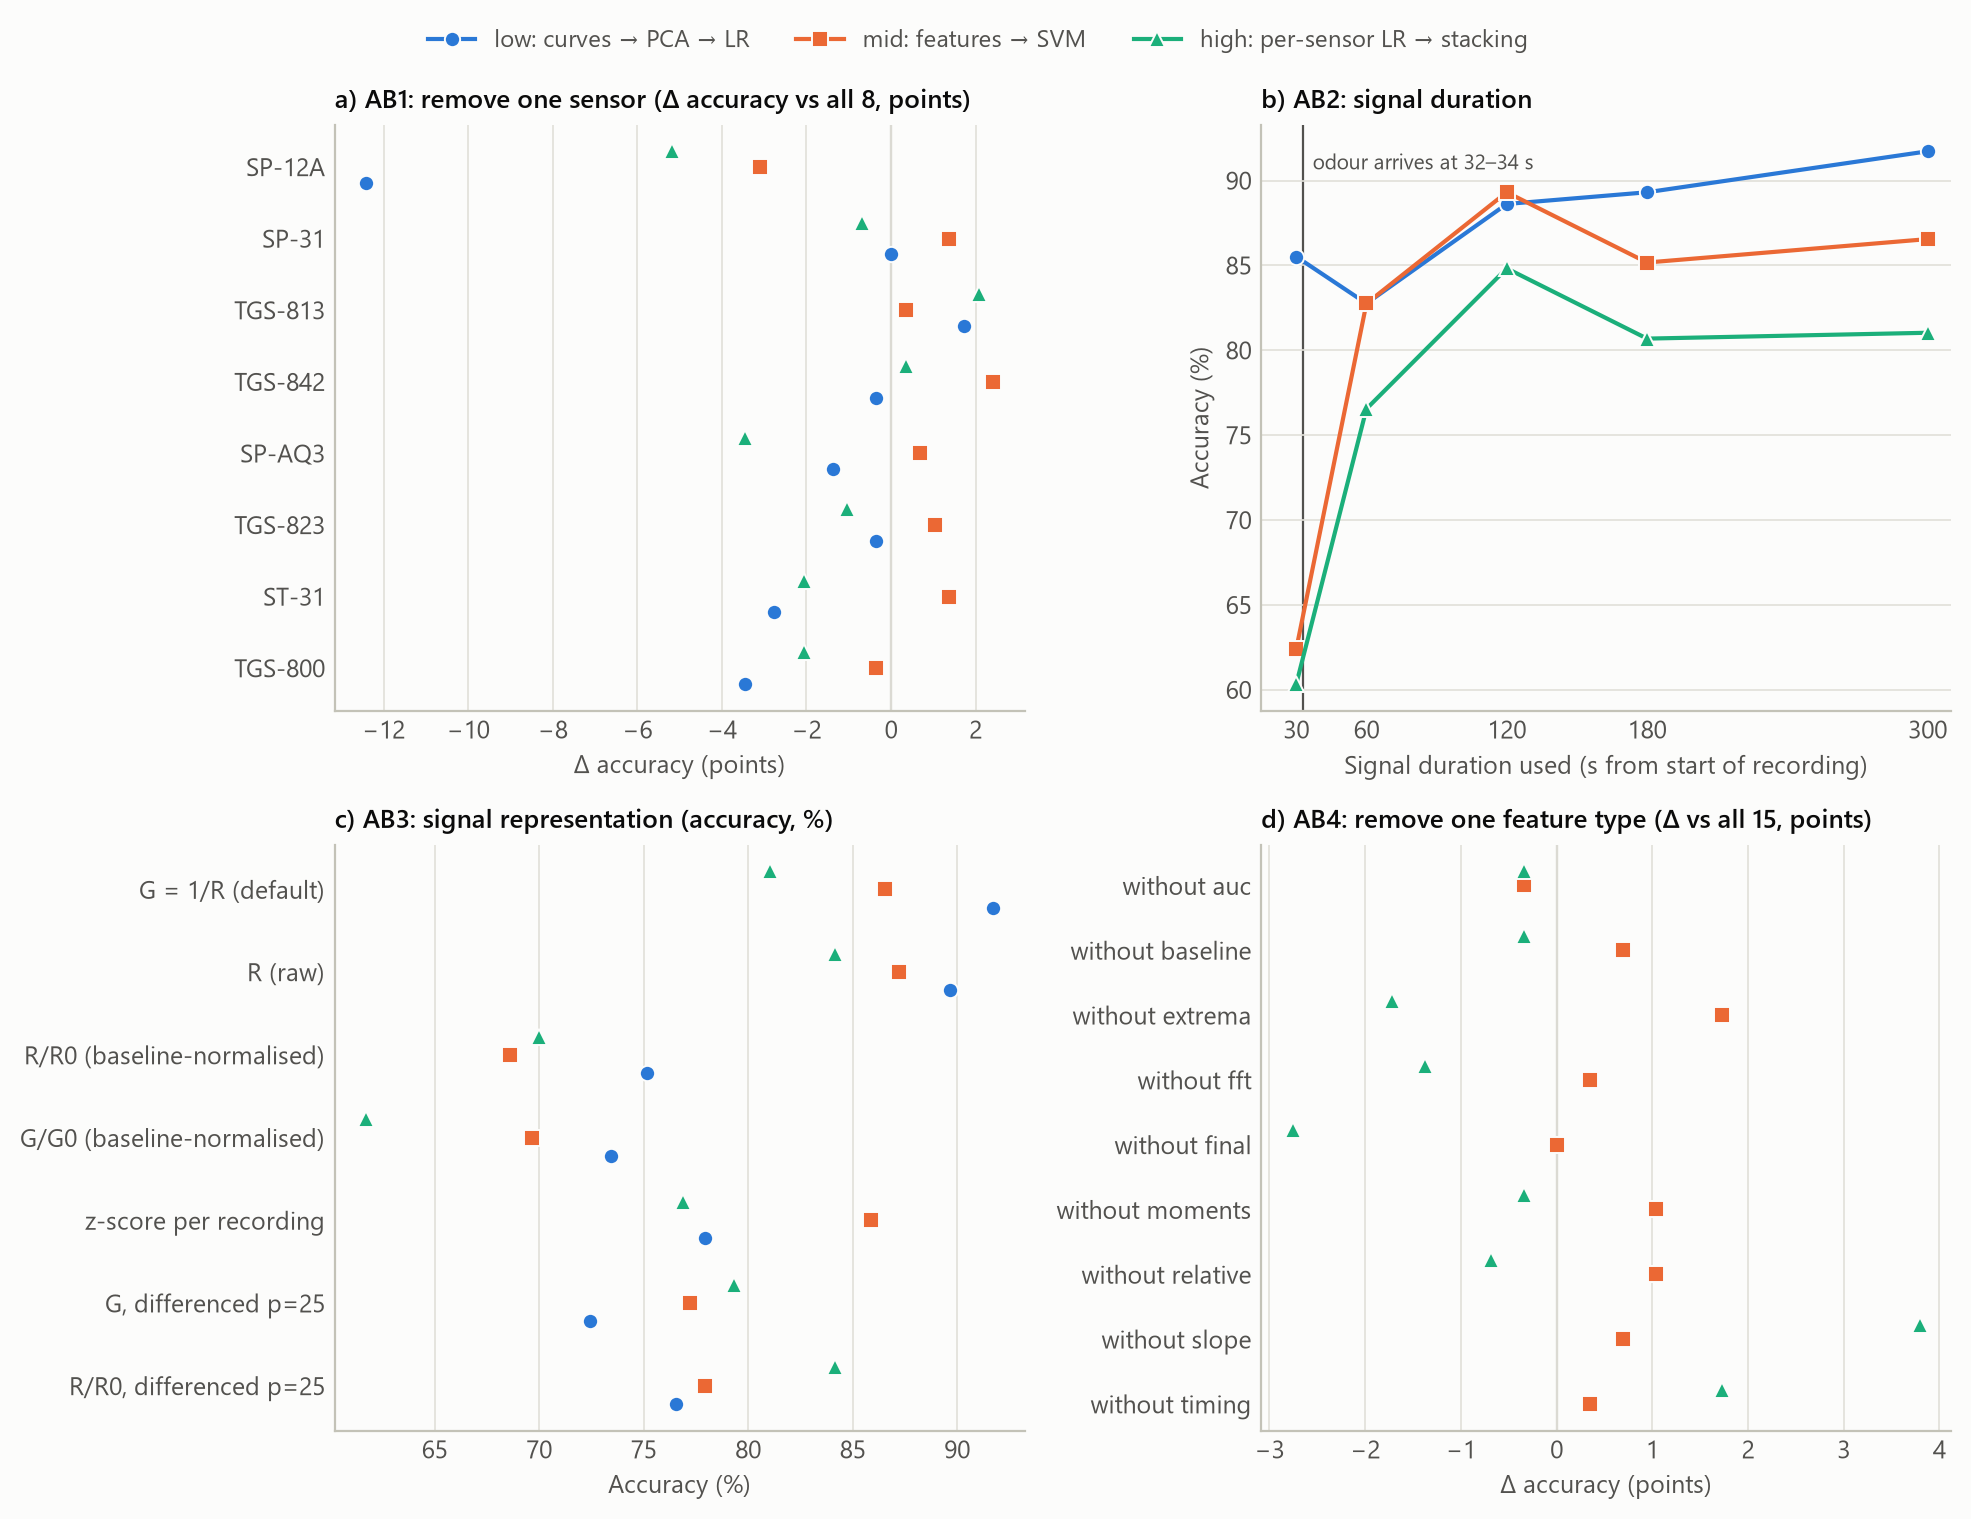
\includegraphics[width=0.9\textwidth]{figures/fig6_s1_ablations.png}
\caption[S1 ablations: sensors, duration, representation and features]{S1 ablations: (a) removal of one sensor; (b) signal duration, with the measured onset of the odour response; (c) signal representation; (d) removal of one feature type.}
\label{fig:ablation}
\end{figure}

\subsection{Experiment B: Fusion of S1 with SmellNet}

Pooling SmellNet into the training data lowers coffee accuracy at every level (Table~\ref{tab:expB}): by 5.2--12.2 points at the mid level (all $p \leq 0.008$) and by 17.2 points with the channel-agnostic CNN ($p = 0.062$ over five repeats), while decision-level fusion at best recovers the S1-only accuracy (77.9\% against 77.2\%, $p = 0.84$). The pooled models did learn SmellNet (32--38\% on its unseen test day in the 50-class task), and even trained on S1 alone the channel-agnostic models lose 4.9--11.3 points against the channel-aware features of Experiment A, which shows the cost of ignoring which sensor produced which signal. AB8 (Table~\ref{tab:ab8}) shows that the loss is not caused by the amount of SmellNet data, since 10\% of the sessions hurt as much ($p \leq 0.006$), whereas the harmonisation steps matter: without the polarity correction the loss of logistic regression doubles ($-$23.6 points), and without per-recording normalisation it reaches $-$37.8 points. Differencing almost removes the loss but also lowers the S1-only models; its single positive difference (MLP, +2.6 points, $p = 0.045$ before correction for the 36 comparisons) leaves the pooled model at 66.7\%, below the S1-only random forest (77.2\%).

\begin{table}[!htbp]
\centering
\caption[Experiment B: S1-only versus S1 + S2 training]{Experiment B: accuracy (\%) on held-out S1 recordings of models trained on S1 only and on S1 + S2 (ten repeats of five-fold cross-validation; five for the CNN). $\Delta$: change against S1 only; $p$: Wilcoxon signed-rank test.}
\label{tab:expB}
\footnotesize
\begin{adjustbox}{max width=\textwidth}
\begin{tabular}{lccccc}
\toprule
\textbf{Model} & \textbf{S1 only (\%)} & \textbf{Pooled S1+S2 (\%)} & \textbf{$\Delta$ (p)} & \textbf{Best decision fusion (\%)} & \textbf{$\Delta$ (p) } \\
\midrule
Logistic regression & 73.4 $\pm$ 2.7 & 61.2 $\pm$ 3.3 & $-$12.2 (0.002) & 75.0 $\pm$ 2.6 [stacking] & +1.6 (0.305) \\
Random forest & 77.2 $\pm$ 3.9 & 72.1 $\pm$ 2.3 & $-$5.2 (0.008) & 77.9 $\pm$ 3.5 [stacking] & +0.7 (0.838) \\
MLP (64 hidden units) & 73.6 $\pm$ 3.8 & 64.0 $\pm$ 3.9 & $-$9.7 (0.004) & 72.8 $\pm$ 4.0 [mean] & $-$0.9 (0.609) \\
Channel-agnostic CNN & 60.7 $\pm$ 3.3 & 43.4 $\pm$ 7.0 & $-$17.2 (0.062) & 62.4 $\pm$ 4.8 [mean] & +1.7 (0.750) \\
\bottomrule
\end{tabular}

\end{adjustbox}
\end{table}

\begin{table}[!htbp]
\centering
\caption[AB8: effect of pooling SmellNet into training]{AB8: S1-only accuracy (\%) and the change (points) caused by pooling SmellNet into training at the mid level (Wilcoxon $p$ in brackets, uncorrected).}
\label{tab:ab8}
\footnotesize
\begin{adjustbox}{max width=\textwidth}
\begin{tabular}{lccc}
\toprule
\textbf{AB8 setting} & \textbf{LR} & \textbf{RF} & \textbf{MLP} \\
\midrule
Full harmonisation, all S2 sessions & 73.4 $\rightarrow$ $-$12.2 (0.002) & 77.2 $\rightarrow$ $-$5.2 (0.008) & 73.6 $\rightarrow$ $-$9.7 (0.004) \\
Only 10\% of S2 sessions & 73.4 $\rightarrow$ $-$13.6 (0.002) & 77.2 $\rightarrow$ $-$11.6 (0.002) & 73.6 $\rightarrow$ $-$8.1 (0.006) \\
No polarity correction (S1 as R) & 73.4 $\rightarrow$ $-$23.6 (0.002) & 69.1 $\rightarrow$ $-$6.2 (0.004) & 73.6 $\rightarrow$ $-$16.2 (0.002) \\
No per-recording normalisation & 71.2 $\rightarrow$ $-$37.8 (0.002) & 77.8 $\rightarrow$ $-$9.3 (0.004) & 79.3 $\rightarrow$ $-$29.3 (0.002) \\
Differenced signals (p = 25) & 66.2 $\rightarrow$ $-$1.2 (0.211) & 73.8 $\rightarrow$ $-$0.5 (0.641) & 64.1 $\rightarrow$ +2.6 (0.045) \\
\bottomrule
\end{tabular}

\end{adjustbox}
\end{table}

\subsection{Experiment C: Fusion within the CQI Database}

Non-sensory data predicts the quality tertile only weakly, and the fusion level hardly matters (Table~\ref{tab:expC}): 49.6 $\pm$ 1.3\% (low), 48.1 $\pm$ 1.5\% (mid) and 49.8 $\pm$ 1.4\% (high), against 33.3\% for chance and 35.9\% for the majority class, with no significant pairwise difference (Wilcoxon $p$ between 0.06 and 0.81). Origin (G3, 48.6\%) carries more signal than bean and physical data (G2, 43.6\%) (AB9); all combiners lie within 1.1 points of each other (AB5); and logistic regression, the SVM and the MLP are ahead of the tree ensembles (AB6). The sensory scores reach 98.1\%, the expected consequence of the total being their sum. S3 also explains what the grades mean (Figure~\ref{fig:cqi}). The classes differ by 0.22--0.34 points per step on every descriptive attribute, and low quality is additionally marked by cup defects: about three times as many category-one defects (0.83 against 0.28 per sample) and nearly twice as many category-two defects (5.04 against 2.73) as high quality, together with lower uniformity, clean-cup and sweetness scores. This is the kind of information an e-nose is designed to capture. The 1.5-point width of the AQ band is smaller than the disagreement between cupping centres \cite{worku2016reproducibility}, which limits how well any instrument can reproduce these grades.

\begin{table}[!htbp]
\centering
\caption[Experiment C: accuracy on the CQI quality tertiles]{Experiment C: accuracy on the quality tertiles of S3 (five repeats of five-fold cross-validation; best model per setting).}
\label{tab:expC}
\footnotesize
\begin{tabular}{llccc}
\toprule
\textbf{Setting} & \textbf{Best model} & \textbf{Accuracy (\%)} & \textbf{Balanced acc. (\%)} & \textbf{Macro-F1} \\
\midrule
C1, low level (G2+G3 concatenated) & SVM & 49.6 $\pm$ 1.3 & 49.1 & 0.480 \\
C2, mid level (per-group PCA) & MLP & 48.1 $\pm$ 1.5 & 47.6 & 0.464 \\
C3, high level (per-group models) & LR, vote & 49.8 $\pm$ 1.4 & 49.6 & 0.487 \\
G2 only (bean/physical) & SVM & 43.6 $\pm$ 1.1 & 43.1 & 0.428 \\
G3 only (origin) & MLP & 48.6 $\pm$ 1.2 & 48.4 & 0.473 \\
Upper bound: G1 sensory scores & LR & 98.1 $\pm$ 0.3 & 98.1 & 0.981 \\
Upper bound: G1+G2+G3 & LR & 96.1 $\pm$ 0.4 & 96.1 & 0.961 \\
\bottomrule
\end{tabular}

\end{table}

\begin{figure}[!htbp]
\centering
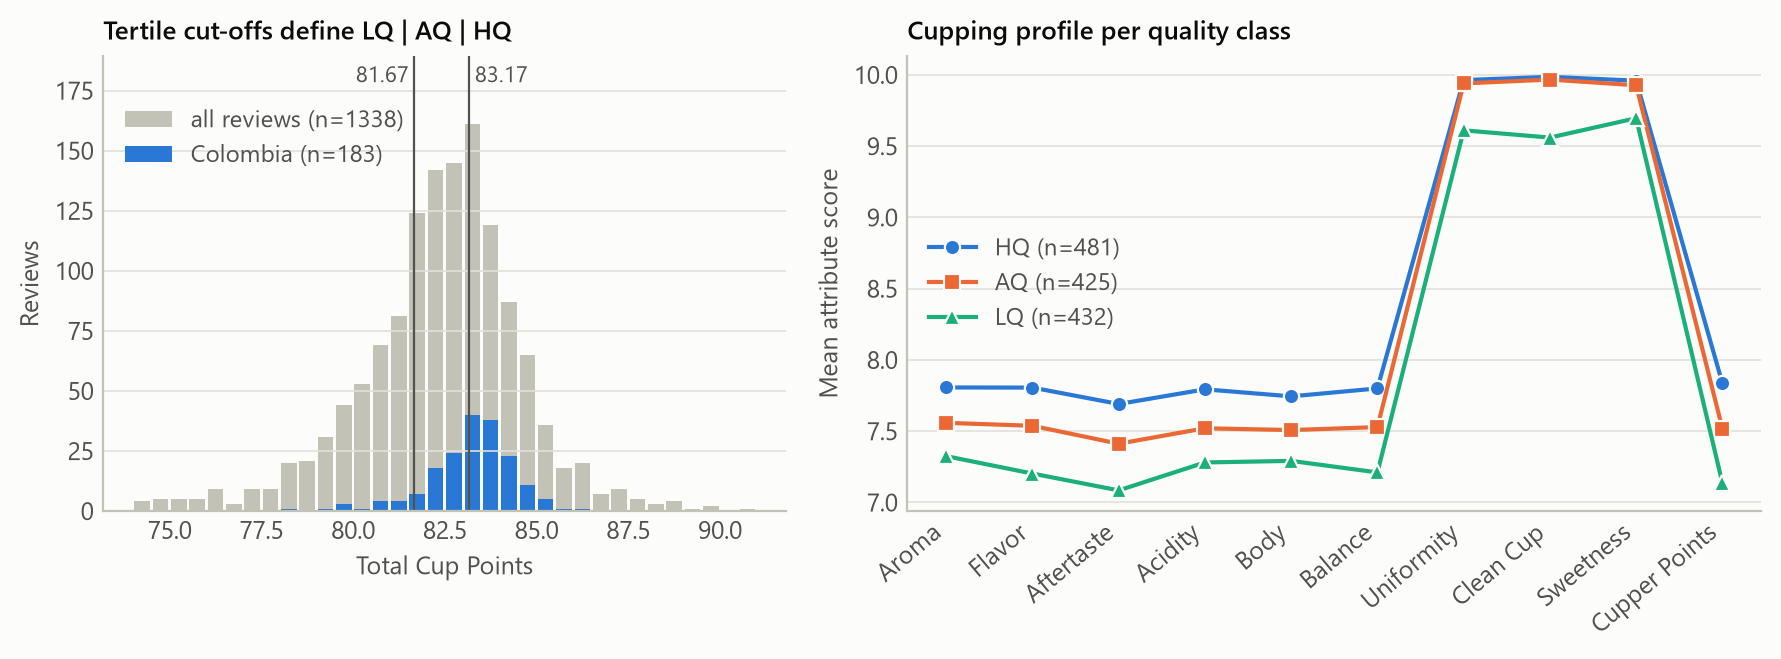
\includegraphics[width=0.9\textwidth]{figures/fig4_cqi_quality_grades.png}
\caption[S3: total cup points and cupping profiles of the quality classes]{S3: distribution of the total cup points with the tertile thresholds (left) and mean cupping profile of each quality class (right).}
\label{fig:cqi}
\end{figure}

\subsection{Experiment D: Fusion of Sensor Data with GC-MS Information}
\label{sec:expD}

Table~\ref{tab:leakage} shows why low-level fusion with class-level chemistry is invalid. Given the GC-MS vector of the true ingredient, a GC-MS-only model and a concatenation of sensor features with GC-MS both reach 100\%; with the only label-free GC-MS input (the average vector), the concatenation falls to 5.2\%, far below the 44.8\% of the same model without GC-MS, so the apparent gain was entirely leakage \cite{kaufman2012leakage}. Among the valid systems (Table~\ref{tab:expD}), contrastive GC-MS training (D1) improves on sensor-only training (D0) in all four settings by 0.9--1.9 points, in the same direction as the 2.2--6.5 points reported in \cite{feng2026smellnet} for this backbone. The joint objective D2 is on par with D0 ($-$0.3 to +1.7 points), and the ensemble D3 adds 1.0--2.2 points in three of the four settings. Differencing ($p = 25$) improves every system, as reported in \cite{feng2026smellnet}, and our absolute accuracies are within 2.3 points of the reported ones in six of the eight D0/D1 settings, although our protocol trains on one day fewer. Masking one channel at test time (AB14) costs 10.4--13.0 points for VOC, CO, NO$_2$ and C$_2$H$_5$OH and about 4 points for alcohol and LPG, and the spectral GC-MS encoding was at least as good as the elemental one (AB12).

\begin{table}[!htbp]
\centering
\caption[Leakage demonstration on SmellNet-Base]{Leakage demonstration on SmellNet-Base (test day 6). The first two systems are invalid by construction.}
\label{tab:leakage}
\footnotesize
\begin{tabular}{lc}
\toprule
\textbf{System (logistic regression, w = 100, p = 25)} & \textbf{Test-day accuracy (\%)} \\
\midrule
GC-MS vector of the true class only (leaky) & 100.0 \\
Sensor features + GC-MS of the true class (leaky) & 100.0 \\
Same model, label-free GC-MS at test time & 5.2 \\
Sensor features only (valid) & 44.8 \\
\bottomrule
\end{tabular}

\end{table}

\begin{table}[!htbp]
\centering
\caption[Experiment D: test-day accuracy of the four systems]{Experiment D: test-day accuracy (\%) of the four systems (mean $\pm$ standard deviation over three seeds) and the values reported in \cite{feng2026smellnet} for the same backbone and settings.}
\label{tab:expD}
\footnotesize
\begin{adjustbox}{max width=\textwidth}
\begin{tabular}{lccccc}
\toprule
\textbf{Window w, period p} & \textbf{D0 sensor-only} & \textbf{D1 contrastive} & \textbf{D2 hybrid} & \textbf{D3 ensemble} & \textbf{Reported D0 / D1 [Feng et al.]} \\
\midrule
w = 50, p = 0 & 20.4 $\pm$ 1.1 & 21.8 $\pm$ 1.0 & 20.2 $\pm$ 0.8 & 19.9 $\pm$ 0.4 & 21.9 / 24.1 \\
w = 50, p = 25 & 24.6 $\pm$ 1.4 & 26.1 $\pm$ 0.8 & 26.2 $\pm$ 1.2 & 25.5 $\pm$ 0.3 & 18.2 / 24.7 \\
w = 100, p = 0 & 21.1 $\pm$ 2.1 & 23.0 $\pm$ 0.9 & 20.8 $\pm$ 2.2 & 23.3 $\pm$ 0.9 & 21.0 / 24.3 \\
w = 100, p = 25 & 25.9 $\pm$ 1.6 & 26.8 $\pm$ 2.7 & 25.9 $\pm$ 2.2 & 27.1 $\pm$ 2.2 & 26.8 / 30.8 \\
\bottomrule
\end{tabular}

\end{adjustbox}
\end{table}

\subsection{Comparison with the Reference Work and Limitations}

Table~\ref{tab:main} compares the results with \cite{rodriguez2010electronic}, whose rows come from different recordings and class definitions. Three points qualify the comparison. First, the public data has a coarser three-class labelling, and its smallest class, AQ, causes most errors. Second, LOO results selected among several variants are optimistic by about 4 points (AB7), so both the reported 92.5--100\% and our 93.1--94.8\% LOO results are upper estimates. Third, not all of the separability is aroma: the 30~s before the odour arrives already give 85.5\%. The absolute static parameter $G_{\max} - G_{\min}$ mixes the response with the pre-exposure conductance ($G_{\min}$ is approximately the baseline conductance for these sensors), whereas the relative form $\Delta G/G_{\min} = R_{\max}/R_{\min} - 1$ is the classical baseline-normalised response, and this level-free form reproduced the method best. On level-free signals, the best estimate of aroma-based quality classification on the public data is 85.9--87.2\% (mid-level fusion of response-shape features), a clear improvement over the reproduced baseline (79.1--80.0\% in repeated cross-validation).

\begin{table}[!htbp]
\centering
\caption[Comparison with the reference work]{Comparison with the reference work. For S1, the accuracy is given as LOO / repeated five-fold cross-validation.}
\label{tab:main}
\footnotesize
\begin{adjustbox}{max width=\textwidth}
\begin{tabular}{llcclcc}
\toprule
\textbf{Method} & \textbf{Data} & \textbf{Classes} & \textbf{Validation} & \textbf{Accuracy (\%)} & \textbf{Macro-F1} & \textbf{Source} \\
\midrule
Rodr\'{\i}guez et al. (2010), analysis 1 & 16 meas. & 4 & LOO & 100 & n/a & reported \\
Rodr\'{\i}guez et al. (2010), analysis 2 & 35 meas. & 9 & LOO & 92.5 & n/a & reported \\
Baseline reproduction ($\Delta$G/Gmin, MLP) & S1, 58 meas. & 3 & LOO / 10$\times$5-fold & 83.3 / 79.1 $\pm$ 3.1 & 0.776 / 0.734 & this work \\
Low-level fusion (A1a, LR) & S1, 58 meas. & 3 & LOO / 10$\times$5-fold & 93.1 / 91.7 $\pm$ 2.1 & 0.907 / 0.896 & this work \\
Low-level fusion (1D-CNN + windows) & S1, 58 meas. & 3 & LOO / 10$\times$5-fold & 93.1 / 89.1 $\pm$ 2.2 & 0.915 / 0.867 & this work \\
Mid-level fusion (A2, SVM) & S1, 58 meas. & 3 & LOO / 10$\times$5-fold & 89.7 / 86.7 $\pm$ 2.2 & 0.857 / 0.830 & this work \\
High-level fusion (A3, SVM, stacking) & S1, 58 meas. & 3 & LOO / 10$\times$5-fold & 86.2 / 84.3 $\pm$ 2.9 & 0.806 / 0.796 & this work \\
S1+S2 fusion (B3, RF, stacking) & S1 + S2 & 3 & 10$\times$5-fold & 77.9 $\pm$ 3.5 & 0.748 & this work \\
Mid-level fusion on level-free (z-scored) signals (SVM) & S1, 58 meas. & 3 & 5$\times$5-fold & 85.9 $\pm$ 4.1 & -- & this work \\
\bottomrule
\end{tabular}

\end{adjustbox}
\end{table}

\textbf{Limitations.} S1 contains only 58 recordings (10 of them AQ), so every estimate carries several points of uncertainty. The pre-exposure sensor levels differ between the classes, and because the release contains no measurement dates or order, their cause (session, ambient conditions, drift or carry-over) cannot be identified. The public labels do not correspond to the classes of the reference work; S1 and S2 share neither sensors nor units; S3 cannot be matched to the sensor recordings; and the GC-MS vectors of S2 are ingredient-level priors from a database rather than measurements of the recorded samples.
\clearpage

%%%***************************************************************************************
\section{Conclusion}
\label{sec:conclusion}

This project reproduced the electronic-nose coffee-quality pipeline of \cite{rodriguez2010electronic} on its public data and compared low-, mid- and high-level data fusion under one leakage-free protocol, using three public data sources.
\begin{enumerate}
\item The PCA view of the reference work is reproduced (99.55\% against 99.62\%) but mainly reflects the scale of one sensor; the literal static parameter barely exceeds the majority class, while its scale-free form reaches 83.3\% LOO (79.1\% in repeated cross-validation).
\item With absolute signals, low-level fusion of the eight sensors is the most accurate (91.7 $\pm$ 2.1\%), ahead of mid-level (86.7\%) and high-level fusion (84.3\%). Much of this advantage, however, comes from sensor levels present before the odour arrives (85.5\% from the first 30~s alone). On level-free signals, mid-level fusion of response-shape features is best (85.9--87.2\%), which is the more trustworthy estimate of aroma-based classification.
\item Fusing a second, heterogeneous gas-sensor data set does not help: pooled training costs 5--17 points because of the sensor mismatch rather than the amount of data, and only decision-level fusion adds it without loss.
\item Non-sensory cupping metadata predicts quality only weakly (about 50\%) at every fusion level; low grades are characterised by cup defects, the attribute an e-nose targets.
\item Class-level GC-MS information must not be fused at the input level, which leaks the label; used for training-time alignment it gives small but consistent gains (+0.9 to +1.9 points), and decision-level combination adds up to 2.2 points.
\item Model selection by LOO on 58 recordings inflated accuracy by about 4 points, so repeated cross-validation should be reported alongside it.
\end{enumerate}

\textbf{Future work.} E-nose data sets should record the measurement session of every sample, randomise the order of samples across classes and apply drift correction \cite{vergara2012chemical}, so that aroma and session effects can be separated. Further directions are extending Experiment D to temporal backbones (convolutional, recurrent and Transformer models), harmonised representations that keep sensor identity across heterogeneous gas-sensor data sets, and sample-level chemical measurements for the coffee recordings.
\clearpage

%%%***************************************************************************************
%\addcontentsline{toc}{section}{References}
%\bibliographystyle{numeric}
\phantomsection
\settocbibname{References}
\bibliography{Myreferences}

%%%%%%%%%%%%%%%%%%%%%%%%%%%%%%%%%%%%%%%%%%%%%%%%%%%%%%%%%%%%%%%%%%%%%%%%%%%%%%%%%%%%%%%%%%%%%%%%%%%%%%%%%
\end{document}
